\documentclass{report}

% \usepackage[greek,english]{babel}
% % 
\usepackage{polyglossia}

\defaultfontfeatures{Mapping=tex-text}
% \setmainfont[Mapping=tex-text]{Liberation Sans } % choose a font that supports greek characters
% \setmainfont[Mapping=tex-text]{GFS Bodoni } % choose a font that supports greek characters Auti tha valw
\setmainfont[Mapping=tex-text]{LiberationSerif} % choose a font that supports greek characters Auti tha valw
\setdefaultlanguage{english}

\setotherlanguage[variant=modern]{greek}

% \newcommand{\tl}{\textlatin}
% \newcommand{\en}{\selectlanguage{english}}
% \newcommand{\gr}{\selectlanguage{greek}}

\usepackage{hyperref}  % package for linking figures etc
\usepackage{enumitem}  % package for description with bullets
\usepackage{graphicx}  % package for importing images
\usepackage{mathtools} % package for math equation
\usepackage{mathrsfs}  % package for math font
\usepackage{indentfirst} % package for getting ident after section or paragraph
\usepackage{subcaption} % package for subfigures
\usepackage[export]{adjustbox}
\usepackage{longtable} % package for multi pages tables
\usepackage{multirow}  % package for tables, multirow
\usepackage{amssymb}
\usepackage{esvect}
\usepackage[
backend=bibtex,
citestyle=authoryear,
% citestyle=authoryear-comp,
% citestyle=authoryear-ibid,
bibstyle=numeric,
sorting=ynt,
% style=numeric,
% style=alphabetic ,
]{biblatex}
\addbibresource{References}

\graphicspath{ {./theory/figures/} }       % path for images

\begin{document}
 
\chapter{Tube Proposal Network}
\section{ Η αρχιτεκτονική του μοντέλου μας}
Σε αυτό το κεφάλαιο, ασχολούμαστε κυρίως με  το Tube Proposal Network (TPN), ένα από τα βασικά στοιχεία του μοντέλου μας ActionNet. Πριν ξεκινήσουμε την
περιγραφήτου, παρουσιάζουμε τη δομή του όλου του μοντέλου μας. Προτείνουμε ένα δίκτυο παρόμοιο με αυτό των \cite{DBLP:journals/corr/HouCS17}.
Η αρχιτεκτονική μας αποτελείται από τα ακόλουθα βασικά στοιχεία:
\begin{itemize}
\item Ένα τρισδιάστατο συνελικτικό μοντέλο (3D Convolutional Network), το οποίο χρησιμοποιείται για την εξαγωγή χαρακτηριστικών.
  Στην υλοποίησή μας χρησιμοποιούμε ένα δίκτυο 3D ResNet34, το οποίο λαμβάνεται από τους \cite{hara3dcnns}  και βασίζεται
  στα ResNet CNNs για  ταξινόμηση εικόνων (\cite{DBLP:journals/corr/HeZRS15}).
\item Το TPN για την εξαγωγή υποψήφιων ToIs (βασιζόμενοι στην ιδέα που παρουσίαζουν οι  \cite{DBLP:journals/corr/HouCS17} ).
\item Έναν ταξινομητή για την εύρεση της κλάσης των προτεινόμενων action video tubes.
\end{itemize}

Η βασική διαδικασία που ακολουθεί το ActionNet είναι:
\begin{enumerate}
\item Δεδομένου ενός βίντεο, το διαχωρίσουμε σε τμήματα βίντεο. Αυτά τα τμήματα βίντεο  σε ορισμένες προσεγγίσεις επικαλύπτονται χρονικά και σε άλλες όχι.
\item Για κάθε τμήμα βίντεο, μετά την εκτέλεση της αλλαγής μεγέθους χωροχρονικά, τροφοδοουμε τα καρέ του στο ResNet34 για να εξάγουμε τους χωροχρονικούς
  χάρτες του. Αυτοί οι χάρτες ενεργοποίησης, στη συνέχεια, τροφοδοτούνται στο TPN για την πρόταση ακολουθιών πλαισίων που πιθανόν περιέχουν κάποια δράση και
  θα τις ονομάσουμε Tubes of Interest (ToIs), όπως κάνουν και οι  \cite{DBLP:journals/corr/HouCS17} .
\item Μετά την πρόταση ToIs για κάθε τμήμα βίντεο, χρησιμοποιώντας έναν αλγόριθμο σύνδεσης, το ActionNet βρίσκει τα τελικά υποψήφια action tubes.
 Αυτά τα action tubes δίνονται ως είσοδο σε έναν ταξινομητή για τον προσδιορισμό της κλάσης τους.
\end{enumerate}

Ένα διάγραμμα του μοντέλου μας ActionNet εμφανίζεται στην εικόνα \ref{fig:whole_network_}. 
\begin{figure}[h]
  % 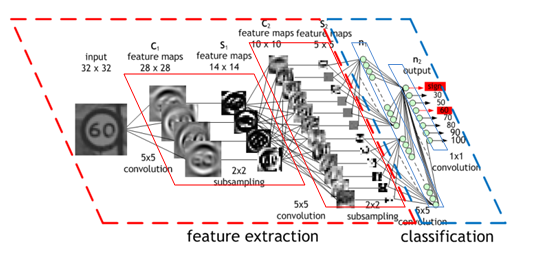
\includegraphics[scale=0.7]{convolutional_neural_network_structure} \]
  \centering
  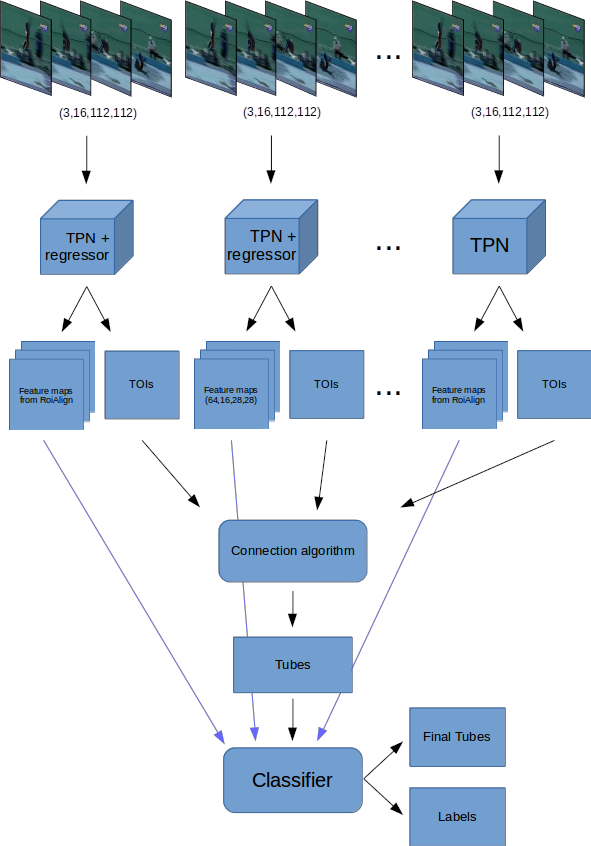
\includegraphics[scale=0.42]{model_prenms}
  \caption{Structure of the whole network}
  \label{fig:whole_network_}
\end{figure}

\section{Εισαγωγή στο  TPN}
Ο κύριος σκοπός του   TPN   είναι να προτείνει \textbf{Tubes of Interest} (TOIs). Αυτά τα   tubes   είναι πιθανό να περιέχουν μια γνωστή δράση και αποτελούνται από μερικά
δυσδιάστατα πλαίσια (1 για κάθε καρέ βίντεο). Το   TPN   έχει εμπνευστεί από το   RPN   που εισήχθη από το    FasterRCNN (\cite{Ren:2015:FRT:2969239.2969250}) ,
αλλά αντί για εικόνες, το   TPN   χρησιμοποιείται σε βίντεο ως κάνουν και οι  \cite{DBLP:journals/corr/HouCS17} . Σε πλήρη αντιστοιχία με τo   RPN  , η δομή
του   TPN   είναι παρόμοια με του   RPN . Η μόνη διαφορά, είναι ότι το   TPN   χρησιμοποιεί   3D Convolutional Layers   και   3D anchors   αντί   2D  .  \par
Σχεδιάσαμε 2 κύριες δομές για τo   TPN . Κάθε προσέγγιση έχει διαφορετικό ορισμό για τα χρησιμοποιούμενα τρισδιάστατa   anchors . 
Η υπόλοιπη δομή του   TPN   είναι κυρίως η ίδια με ορισμένες μικρές διαφορές στο στάδιο του    regression.   \par

\section{Προετοιμασία πριν το TPN}

\subsection{Η προετοιμασία των δεδομένων}
Πριν εισαχθεί ένα βίντεο στο   ResNet   και στο   TPN   για να εξαγάγουμε τα χαρακτηριστικά του και πιθανά   ToIs  , αυτό το βίντεο πρέπει να προεπερξαστεί.
Η διαδικασία προεπεξεργασίας είναι η ίδια και για τις δύο προσεγγίσεις του TPN.
Η αρχιτεκτονική μας λαμβάνει ως είσοδο μια ακολουθία από σταθερό αριθμό καρέ  που έχουν σταθερό πλάτος και ύψος. Ωστόσο, κάθε βίντεο είναι πιθανόν να έχει διαφορετική ανάλυση. Αυτό δημιουργεί
την ανάγκε να αλλάξουμε  το μέγεθος κάθε πλαισίου πριν εισαχθούν στο ActionNet. Όπως αναφέρθηκε στο προηγούμενο κεφάλαιο, το πρώτο στοιχείο του δικτύου μας είναι ένα   3D RenNet  
που υλοποιήθηκε από τους   \cite{hara3dcnns}. Αυτό το δίκτυο έχει σχεδιαστεί να δέχεται βίντεο  με διαστάσεις (112, 112).
Ως αποτέλεσμα, μεταβάλλουμε  το μέγεθος κάθε καρέ από τα βίντεο των dataset σε (112, 112). Για να διατηρήσουμε την αναλογία διαστάσεων, προσθέτουμε μηδενικές τιμές 
αριστερά και δεξιά, είτε πάνω και κάτω, ανάλογα με το ποια διάσταση είναι μεγαλύτερη. Στο σχήμα  \ref{fig:Preprocess_example} μπορούμε να δούμε το αρχικό πλαίσιο και το μέγεθος και το ενισχυμένο.
Σε πλήρη αντιστοιχία, αλλάζουμε και το μέγεθος των πραγματικών πλαισίων οριοθέτησης αληθείας για κάθε καρέ (Τα σχήματα \ref{fig:original_image_rois}  και \ref{fig:trans_image_rois} το απεικονίζουν).

\begin{figure}[h]
  \centering
  \begin{subfigure}{0.35\textwidth}
    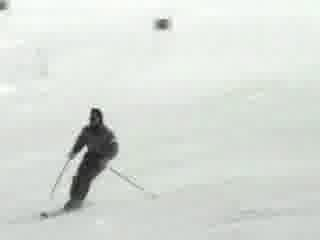
\includegraphics[width=\textwidth]{./figures/original_image.jpg}
    \caption{}
    \label{fig:original_image}
   \end{subfigure}
  \hfill
  \begin{subfigure}{0.35\textwidth}
    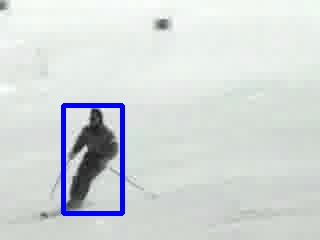
\includegraphics[width=\textwidth]{./figures/original_image_rois.jpg}
    \caption{}
    \label{fig:original_image_rois}
  \end{subfigure}
  \hfill
  \begin{subfigure}{0.35\textwidth}
    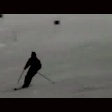
\includegraphics[width=\textwidth]{./figures/transformed_image.jpg}
    \caption{}
    \label{fig:trans_image}
  \end{subfigure}
  \hfill
  \begin{subfigure}{0.35\textwidth}
    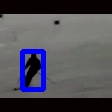
\includegraphics[width=\textwidth]{./figures/transformed_image_rois.jpg}
    \caption{}
    \label{fig:trans_image_rois}
  \end{subfigure}

  \caption{ At (a), (b) frame is its original size and at (c), (d) same frame after preprocessing part}
  \label{fig:Preprocess_example}
\end{figure}

\subsection{3D ResNet}
Πριν από τη χρήση του Tube Proposal Network, εξάγουμε  χωροχρονικά χαρακτηριστικά από το βίντεο. Για να γίνει αυτό, εξάγουμε τα 3 πρώτα στρώματα ενός
προεκπαιδευμένο 3D ResNet34. Αυτό το μοντέλο είναι προεκπαιδευμένο στο Kinetics dataset (\cite{DBLP:journals/corr/KayCSZHVVGBNSZ17}) για τη διάρκεια του δείγματος ίση με
16 καρέ και μέγεθος δείγματος ίσο με (112, 122).  \par
Αυτό το δίκτυο συνήθως χρησιμοποιείται για την ταξινόμηση ολόκληρου του βίντεο, οπότε μερικά από τα στρώματα του χρησιμοποιούν temporal stride ίσο με 2.
Εμείς, όμως, θέτουμε το temporal stride  ίσο με 1 γιατί δεν θέλουμε να χάσουμε χρονικές πληροφορίες κατά τη διάρκεια της διαδικασίας.
Έτσι, η έξοδος του τρίτου στρώματος είναι ένα χάρτης χαρακτηριστικών με διαστάσεις (256, 16, 7, 7). Τροφοδοτουμε αυτό τον χάρτη  χαρακτηριστιών στο TPN,
το οποίο περιγράφεται στις ακόλουθες ενότητες.

\section{Τα τριασδιάστατα  anchors ως  6-dim διανύσματα}
\subsection{Πρώτη περιγραφή}
Ξεκινήσαμε να σχεδιάζουμε το TPN εμπνευσμένοι από την δουλειά των \cite{DBLP:journals/corr/HouCS17}. Έτσι, θεωρούμε κάθε anchor ως ένα
τρισδιάστατο πλαίσιο  το οποίο γράφεται ως $(x_1, y_1, t_1, x_2, y_2, t_2)$ όπου $x_1, y_1, t_1$ είναι
οι πάνω μπροστά αριστερές διαστάσεις του κύβου και $x_2, y_2, t_2$ είναι οι κάτω πίσω δεξιά όπως φαίνεται και στην εικόνα \ref{fig:anchor_6d}.
\begin{figure}[h]
  \centering
  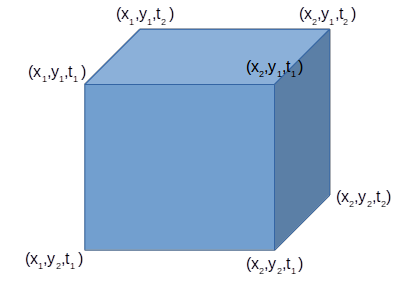
\includegraphics[scale=0.5]{anchor_6d}
  \caption{An example of the anchor $(x_1,y_1,t_1,x_2,y_2,t_2)$}
  \label{fig:anchor_6d}
\end{figure}

Το κύριο πλεονέκτημα αυτής της προσέγγισης είναι ότι εκτός από τις διαστάσεις x-y, η διάσταση του χρόνου είναι μεταβαλλόμενη. Ως αποτέλεσμα, οι προτεινόμενες ΤοΙs
δεν έχουν καθορισμένη χρονική διάρκεια. Αυτό θα μας βοηθήσει να ασχοληθούμε με τα μη-κομμένα (untrimmed) βίντεο, επειδή τα προτεινόμενα TOIs θα μπορούν να εξαιρέσουν background καρέ.
Για αυτήν την προσέγγιση, χρησιμοποιούμε \textbf{n = 4K = 60} anchors για κάθε pixel στους χάρτες ενεργοποίησης του TPN. Έχουμε k anchores για κάθε διαφορετική διάρκεια anchor
 (5 κλίμακες των 1, 2, 4, 8, 16, 3 αναλογίες διαστάσεων 1:1, 1:2, 2:1 και 4 διάρκειες 16, 12, 8, 4 καρέ).
Στο \cite{DBLP:journals/corr/HouCS17}, τα anchors του δικτύου ορίζονται σύμφωνα με τα πιο συνηθισμένα anchors του συνόλου δεδομένων. Αυτό, ωστόσο,
δημιουργεί την ανάγκη επανασχεδιασμού του δικτύου για κάθε σύνολο δεδομένων. Στην προσέγγισή μας, χρησιμοποιούμε τα ίδια anchors και για τα δύο σύνολα δεδομένων, επειδή θέλουμε το δίκτυό μας να μην
να βασίζεται στο σύνολο δεδομένων, αλλά να είναι σε θέση να γενικευσει για διάφορα σύνολα δεδομένων. Ως διάρκεια δειγματοληψίας, επιλέξαμε 16 καρέ ανά τμήμα βίντεο, επειδή
η προ-εκπαιδευμένη έκδοση ResNet που χρησιμοποιούμε έχει εκπαιδευτεί για βίντεο κλιπ με αυτή τη διάρκεια.
Έτσι, η δομή του TPN είναι:
\begin{itemize}
\item 1 3D Convolutional Layer με kernel size = 3, stride = 3 και padding = 1
\item 1 classification layer που εξάγει \textit{2n scores} για το αν υπάρχει ή όχι δράση για \textit{n tubes}.
\item 1 regression layer που εξάγει \textit{6n διαστάσεις} ($x_1,y_1,t_1,x_2,y_2,t_2$) για \textit{n tubes}.
\end{itemize}

Η δομή του TPN παρουσιάζεται στην Εικόνα \ref{fig:tpn_1_1}. Το αποτέλεσμα του TPN είναι τα k-καλύτερα κουτιά, τα οποία
είναι τα πιο πιθανά να περιέχουν κάποια δράση.
\begin{figure}[h]
  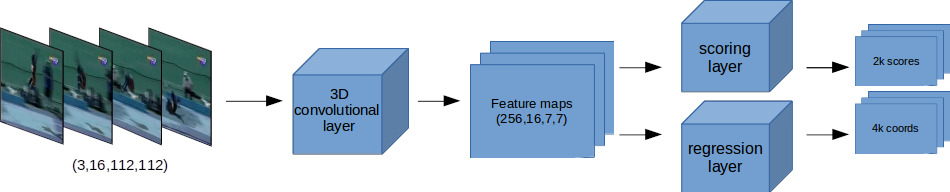
\includegraphics[width=1.\textwidth]{tpn_1_1}
  \caption{Structure of TPN}
  \label{fig:tpn_1_1}
\end{figure}

\subsection{Training}
Όπως προαναφέρθηκε, το TPN εξάγει ToIs ως 6-διάστατα διανύσματα. Για το λόγο αυτό, τροποποιήσαμε τα πραγματικά πλαίσια ανά καρέ σε πραγματικά Tubes.
Θεωρούμε δεδομένο ότι το άτομο που δρα, δεν μπορεί να κινηθεί πολύ σε 16 καρέ, γι ' αυτό χρησιμοποιούμε τέτοιου είδους Tubes. Όπως φαίνεται 
στο σχήμα \ref{fig:gt_tubes_and_rois}, αυτά τα tubes είναι τρισδιάστατα κουτιά που περιλαμβάνουν όλα τα πραγματικά πλαίσια, τα οποία είναι διαφορετικά
ανά καρέ.
\begin{figure}[h]
  \centering
  \begin{subfigure}{0.15\textwidth}
    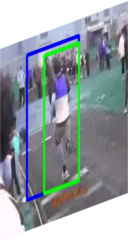
\includegraphics[width=\textwidth]{output/img_0.jpg}
  \end{subfigure}
  \begin{subfigure}{0.15\textwidth}
    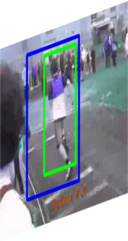
\includegraphics[width=\textwidth]{output/img_3.jpg}
  \end{subfigure}
  \begin{subfigure}{0.15\textwidth}
    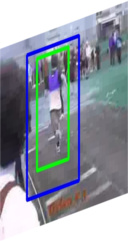
\includegraphics[width=\textwidth]{output/img_5.jpg}
  \end{subfigure}
  \begin{subfigure}{0.15\textwidth}
    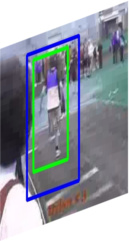
\includegraphics[width=\textwidth]{output/img_7.jpg}
  \end{subfigure}
  \begin{subfigure}{0.15\textwidth}
    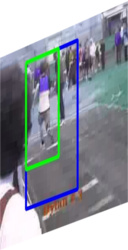
\includegraphics[width=\textwidth]{output/img_11.jpg}
  \end{subfigure}
  \begin{subfigure}{0.15\textwidth}
    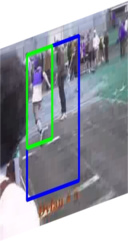
\includegraphics[width=\textwidth]{output/img_15.jpg}
  \end{subfigure}
  \caption{Το πραγματικό tube έχει μπλε χρώμα και το πραγματικό ανά καρέ πλαίσιο έχει χρώμα πράσινο}
  \label{fig:gt_tubes_and_rois}
\end{figure}

Για τη διαδικασία training, για κάθε βίντεο, επιλέγουμε τυχαία ένα μέρος του, το οποίο έχει διάρκεια 16 καρέ. Θεωρούμε ένα anchor ως πρώτο πλάνο, αν η βαθμολογία επικάλυψης του με το πραγματικό
tube είναι μεγαλύτερη από 0.5 . Διαφορετικά, θεωρείται ως anchor φόντου. Χρησιμοποιούμε έναν scoring layer για να ταξινομήσουμε σωστά αυτά τα anchors και χρησιμοποιούμε
την Cross Entropy Loss ως συνάρτηση κόστους (loss function). Έχουμε πολλά anchors για να προτείνουμε μια δράση, αλλά μικρό αριθμό δράσεων σε κάθε βίντεο, έτσι επιλέγουμε 256 anchors συνολικά για
κάθε batch. Ορίζουμε ότι o μέγιστος αριθμός των anchors προσκηνίου να είναι 25\% από τους 256 anchors και τα υπόλοιπα είναι anchors φόντου.  \par
Η σωστή ταξινόμηση ενός anchor δεν είναι αρκετή για να προτείνουμε ToIs. Είναι, επίσης,  απαραίτητο τα anchors να επικαλύπτονται όσο το δυνατόν περισσότερο με τα πραγματικά tubes.
Αυτός είναι ο λόγος που χρησιμοποιούμε ένα επίπεδο παλινδρόμησης. Αυτό το layer "κινεί" τον κύβο στην περιοχή που πιστεύεται ότι είναι πιο κοντά στη δράση.
Για συνάρτηση κόστους παλινδρόμησης χρησιμοποιούμε την συνάρτηση κόστους smooth-L1  όπως παρουσιάζεται από τους \cite{DBLP:journals/corr/GirshickDDM13}. Για να υπολογίσομε τους
 στόχους παλινδρόμησης, χρησιμοποιούμε την pytorch εφαρμογή του  FasterRCNN (\cite{jjfaster2rcnn}) για την παλινδρόμηση του πλαισίου και 
τροποποιούμε τον κώδικα επεκτείνοντας τον για 3 διαστάσεις. % Doobf{για περισσότερες πληροφορίες}
Έτσι έχουμε:

\[ \begin{matrix}
    t_x = (x-x_a)/w_a, & t_y = (y-y_a)/h_a, & t_z= (z-z_a)/d_a, \\
    t_w= log(w/w_a), & t_h= log(h/h_a), & t_d = log(d/d_a), \\
    t^*_x = (x^* - x_a)/w_a, & t^*_y = (y^* - y_a)/h_a, & t^*_z = (z^* - z_a)/d_a, \\
    t^*_w = log(w^* /w_a), & t^*_h = log(h^*/h_a), & t^*_d = log(d^*/d_a),
    % t∗x= (x∗−xa)/wa,  t∗y= (y∗−ya)/ha,t∗w= log(w∗/wa),  t∗h= log(h∗/ha)
  \end{matrix}
\]
όπου τα \textit{x, y, z, w, h, d} υποδεικνύουν τις συντεταγμένες του κέντρου του τρισδιάστατου κουτιού καθώς επίσης το πλάτος, το ύψος και τη διάρκειά του. Οι μεταβλητές
$x, x_a, \text{ and } x^*$ αφορούν το προβλεπόμενο πλαίσιο, το πλαίσιο του anchor και το πραγματικό πλαίσιο αντίστοιχα (ομοίως για \textit{y, z, w, h, d}). Φυσικά, υπολογίζουμε την
απώλεια παλινδρόμησης μόνο για τα anchors προσκηνίου και όχι αυτά του φόντου, συνεπώς στην χειρότερη θα υπολογίσουμε 64 στόχους για κάθε batch. \par

Για να συνοψίσουμε τη διαδικασία training, εκπαιδεύουμε 2 layers για το TPN, scoring  και reggression. Η συνάρτηση κόστους περιλαμβάνει τα
training losses που προκύπτους απ' αυτά τα layers και ο τύπος της είναι:
% \[ L  = \frac{1}{N_{cls}} \sum_iL_{cls}(p_i, p^*) + \frac{1}{N_{reg}}\sum_ip_i^*L_{reg}(t_i,t_i^*) \]
\[ L  =  \sum_iL_{cls}(p_i, p_i^*) + \sum_ip_i^*L_{reg}(t_i,t_i^*) \]
όπου:
\begin{itemize}
\item $L_{cls} $ είναι η Cross Entropy loss που χρησιμοποιούμε γαι να εκπαιδεύσουμε τα anchors, με $p_i$ είναι η προβλεπόμενη κλάση, $p_i^*$ είναι η πραγματική κλάση και
  $p_i, p_i^* \in \{0,1\}$
\item $L_{reg} $ είναι η συνάρτηση κόστους smooth-L1, η οποία πολλαπλασιάζεται με $p_i^*$ προκείμενου να ενεργοποιείται όταν υπάρχει θετικό anchor $(p_i^* = 1)$
  και να απερνεργοποιείται για τα background anchors $(p_i^* = 0)$.
\end{itemize}

\subsection{Validation}

Η διαδικασία validation είναι κάπως παρόμοια με τη διαδικασία training.
Επιλέγουμε τυχαία 16 καρέ από ένα βίντεο επικύρωσης και εξετάζουμε αν υπάρχει τουλάχιστον 1 προτεινόμενο ΤοΙ
που επικαλύπτει $\ge$ 0,5 με κάθε πραγματικό tube και παίρνουμε το recall score.
Για να λάβουμε καλές προτάσεις, μετά τη λήψη των classification scores και των regression targets από το
αντίστοιχα layers, χρησιμοποιούμε τον αλγόριθμο Non-Maximum Suppresion(NMS).  Έχουμε ορίσει το κατώφλι του NMS ίσο με 0,7 
και κρατάμε τους πρώτους 150 κύβους με τη μεγαλύτερη βαθμολογία.
\subsection{Modified Intersection over Union(mIoU) } 
Κατά τη διάρκεια της προπόνησης, έχουμε πολλά anchors. Πρέπει να τα ταξινομήσουμε ως anchors προσκηνίου ή
anchors παρασκηνίου. Τα anchors προσκηνίου είναι εκείνα που περιέχουν κάποια ενέργεια και, αντίστοιχα, του φόντου
που δεν έχουν. Όπως παρουσιάστηκε προηγουμένως, το IoU για τα cuboids υπολογίζει το ποσοστό μεταξύ του όγκου της επικάλυψης
και του όγκου των Ένωσης.
Διαισθητικά, αυτό το κριτήριο είναι καλό για την αξιολόγηση του βαθμού επικάλυψης 2 tube, αλλά έχει ένα μεγάλο μειονέκτημα:
Θεωρεί ότι οι διαστάσεις x-y έχουν την ίδια σημασία με τη χρονική διάσταση, τo οποίo δεν επιθυμούμε. Κι αυτό  διότι
πρώτον, μας ενδιαφέρει να είμαστε ακριβείς στη χρονική διάσταση, και στη συνέχεια μπορούμε να διορθώσουμε τον τομέα x-y.
Ως αποτέλεσμα, αλλάζουμε τον τρόπο με τον οποίο υπολογίζουμε το Intersection over Union. Υπολογίζουμε ξεχωριστά
το IoU στις διαστάσεις χ-y (IoU-xy) και στην t διάσταση (IoU-t). Τέλος,  πολλαπλασιάζουμε αυτά τα δύο score για να πάρουμε το τελικό IoU.
Συνεπός ο τύπος για 2 tubes ($x_1, y_1, t_1, x_2, y_2, t_2$) and ($x'_1, y'_1, t'_1, x'_2, y'_2, t'_2$) είναι:
\[ IoU_{xy} = \frac{ \text{Area of Overlap in x-y}} { \text{Area of Union in x-y}}  \]
\[ IoU_t = \frac { max(t_1, t'_1) - min(t_2, t'_2)} {min(t_1,t'_1) - max(t_2,t'_2)} \]
\[ IoU = IoU_{xy} \cdot  IoU_t \]
Το παραπάνω κριτήριο μας βοηθά να εξισορροπήσουμε τις επιπτώσεις του χρόνου στο IoU score. Για παράδειγμα, ας εξετάσουμε 2 anchors:
a = (22, 41, 1, 34, 70, 5) και b = (20, 45, 2, 32, 72, 5). Αυτά τα 2 anchor στις διαστάσεις  x-y έχουν βαθμολογία IoU ίσο με 0,61.
Αλλά δεν είναι ακριβώς επικαλυπτόμενα στην διάσταση του χρόνου. Χρησιμοποιώντας την πρώτη προσέγγιση έχουμε 0,5057 IoU βαθμολογία ενώ η
δεύτερη προσέγγιση μας δίνει 0,4889. Έτσι, το δεύτερο κριτήριο θα απέρριπτε αυτό το anchor, διότι υπάρχει μια διαφορά στην χρονική διάρκεια. \par


Για να επιβεβαιώσουμε την ιδέα μας, εκπαιδεύουμε το TPN χρησιμοποιώντας τόσο το IoU κριτήριο όσο και το mIoU  για την επικάλυψη των tubes. Στο πίνακα \ref{table:iou_miou}
μπορούμε να δούμε την απόδοση σε κάθε περίπτωση και για τα δύο σύνολα δεδομένων, JHMDB και UCF. Το recall όριο για αυτή την περίπτωση είναι 0,5 και κατά την διάρκεια του
validation χρησιμοποιούμε το κανονικό IoU για να καθορίσουμε αν 2 tubes επικαλύπτονται.
\begin{table}[h]
\centering
  \begin{tabular}{|| c | c || c ||}
    \hline
    \textbf{Dataset} & \textbf{Criterion} & \textbf{Recall(0.5)} \\
    \hline  \hline
    \multirow{2}{4em}{JHMDB} & IoU & 0.70525 \\
    \cline{2-3}
    {} & mIoU & 0.7052 \\
    \hline
    \multirow{2}{4em}{UCF} & IoU & 0.4665 \\
    \cline{2-3}
    {} & mIoU & 0.4829 \\
    \hline      
  \end{tabular}
  \caption{Recall results for both datasets using IoU and mIoU metrics}
  \label{table:iou_miou}
\end{table}

Ο πίνακας  \ref{table:iou_miou} μας δείχνει ότι το τροποποιημένο-IoU μας δίνει ελαφρώς καλύτερη απόδοση recall μόνο στο σύνολο δεδομένων UCF. Αυτό είναι λογικό, επειδή το σύνολο δεδομένων JHMDB
χρησιμοποιεί κομμένα βίντεο, συνεπώς  η χρονική διάρκεια δεν επηρεάζει πολύ. Έτσι, από τώρα και στο εξής, κατά τη διάρκεια του training χρησιμοποιούμε το mIoU ως επικαλυπτόμενη πολιτική βαθμολογίας.

\subsection{Βελτιώνοντας το  TPN score}
Μετά την πρώτη δοκιμή, μας ήρθε η  ιδέα ότι σε ένα βίντεο που διαρκεί 16 καρέ, στον τομέα του χρόνου, όλα τα είδη των ενεργειών μπορούν να χωρίζονται στις ακόλουθες κατηγορίες:
\begin{enumerate}
\item Η ενέργεια ξεκινά από το n-ο πλαίσιο και ολοκληρώνεται μετά το 16th καρέ του βίντεο που έχει υποβληθεί σε δειγματοληψία.
\item Η ενέργεια έχει ήδη ξεκινήσει πριν από το 1η καρέ του βίντεο και τελειώνει στο n-th πλαίσιο.
\item Η ενέργεια έχει ήδη ξεκινήσει πριν από το 1η καρέ του βίντεο και ολοκληρώνεται μετά το 16th καρέ βίντεο.
\item Η ενέργεια ξεκινά και τελειώνει σε αυτά τα 16 καρέ του βίντεο.
\end{enumerate}

Επιπλέον, παρατηρήσαμε ότι οι περισσότερες ενέργειες, στα σύνολα δεδομένων μας, διαρκούν περισσότερο από 16 καρέ. Έτσι, ήρθαμε με την ιδέα να προσθέσουμε 1 scoring layer και 1 reggression Layer
που θα προτείνει ToIs με σταθερή διάρκεια ίση με τη διάρκεια του δείγματος (16 καρέ) και θα λάβει υπόψη τις χωρικές πληροφορίες που παράγονται από τους χάρτες ενεργοποίησης.
Η νέα δομή του TPN εμφανίζεται στην εικόνα \ref{fig:tpn_1_2}. Αφού λάβουμε τις προτάσεις και από και από τα δύο scoling layers, τις ενώνουμε με ποσοστό 1:1 μεταξύ των ToI που
εξαχθήκαν από τα δύο υποδίκτυα.
\begin{figure}[h]
  \centering
  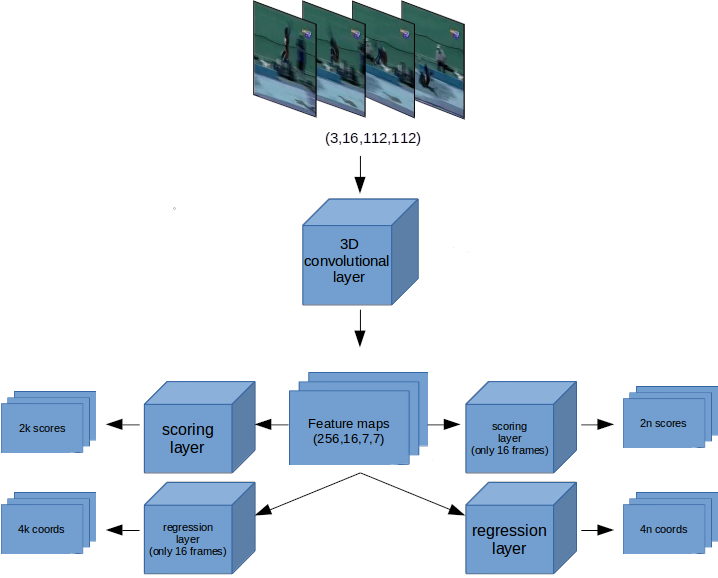
\includegraphics[scale=0.5]{tpn_1_2}
  \caption{TPN structure after adding 2 new layers, where k = 5n.}
  \label{fig:tpn_1_2}
\end{figure}
Στόχος μας είναι να «συμπιέσουμε» τους χάρτες της χρονικής διάστασης, προκειμένου να προτείνουμε ΤοΙs σύμφωνα μόνο με τις χωρικές πληροφορίες.
Έτσι, βρίκαμε με 2 τεχνικές για να πραγματοποιήσουμε κάτι τέτοιο:
\begin{enumerate}
\item Να χρησιμοποιήσουμε  3D Convolutional Layers με μέγεθος πυρήνα = (διάρκεια δείγματος, 1, 1), stride = 1 και χωρίς padding για scoring και regression.
  Αυτός ο πυρήνας «κοιτάει» μόνο στη χρονική διάσταση των χαρτών ενεργοποίησης και δεν θεωρεί καμία χωρική εξάρτηση.
\item Nα αποκτήσΟυμε τις μέσες τιμές από τη χρονική διάσταση και στη συνέχεια να χρησιμοποιήσουμε ένα 2D Convolutional Layer για scoring και regression.
\end{enumerate}

% \textbf{TODO na perigrapsw oti thelw na exw ola ta xronika features}
\par
Οι διαδικασίες training και validation παραμένουν ίδιες. Η μόνη μεγάλη διαφορά είναι ότι τώρα έχουμε κόστη  από 2 διαφορά σύστημα που προτείνουν TOIs. Έτσι, κατα την διάρκεια του validation,
εμείς αρχικά, ενώνουμε τα προτεινόμενα ToIs και, στη συνέχεια, ακολουθούμε την ίδια διαδικασία, η οποία είναι να υπολογίσουμε το recall. Για το training loss, έχουμε 2 διαφορετικές
Cross-entropy loss συναρτήσεις και 2 διαφορετικά smooth-L1 losses. Έτσι, η απώλεια εκπαίδευσης, τώρα, ορίζεται ως:

  % \begin{aligned}
 % L  =  \sum_iL_{cls}(p_i, p_i^*) + \sum_iL_{cls}(p_{fixed,i}, p_{fixed,i}^*) +  
 %  \sum_ip_i^*L_{reg}(t_i,t_i^*) + \sum_ip_{fixed,i}^*L_{reg}(t_{fixed,i},t_{fixed,i}^*) 
% L  =2


% \[ L  =  \sum_iL_{cls}(p_i, p_i^*) + \sum_iL_{cls}(p_{fixed,i}, p_{fixed,i}^*) +  \newline
%   \sum_ip_i^*L_{reg}(t_i,t_i^*) + \sum_ip_{fixed,i}^*L_{reg}(t_{fixed,i},t_{fixed,i}^*) \]
% \end{aligned}


\begin{equation} 
\begin{split}
 L  =  \sum_iL_{cls}(p_i, p_i^*) + \sum_iL_{cls}(p_{fixed,i}, p_{fixed,i}^*) + \\
   \sum_ip_i^*L_{reg}(t_i,t_i^*) + \sum_ip_{fixed,i}^*L_{reg}(t_{fixed,i},t_{fixed,i}^*) 
  % \sum_iL_{cls}(p_i, p_i^*) + \sum_iL_{cls}(p_{fixed,i}, p_{fixed,i}^*) 
\end{split}
\end{equation}

όπου:
\begin{itemize}
  \item $L_{cls} $ είναι η Cross Entropy loss που χρησιμοποιούμε γαι να εκπαιδεύσουμε τα anchors, με $p_i$ είναι η προβλεπόμενη κλάση, $p_i^*$ είναι η πραγματική κλάση και
  $p_i, p_i^* \in \{0,1\}$
\item $L_{reg} $ είναι η συνάρτηση κόστους smooth-L1, η οποία πολλαπλασιάζεται με $p_i^*$ προκείμενου να ενεργοποιείται όταν υπάρχει θετικό anchor $(p_i^* = 1)$
  και να απερνεργοποιείται για τα background anchors $(p_i^* = 0)$.
\item $p_i $ είναι τα anchors από τα scoring και regression layers με μεταβλητή χρονική διάρκιεα και  $p_i^*$ είναι η αντίστοιχη πραγρατική τους κλάση.
\item $p_{fixed,i} $ είναι τα anchors από τα scoring και regression layers με σταθερή χρονική διάρκεια ίση με 16 καρέ και $p_{fixed,i}^*$ είναι η αντίστοιχη πραγματική του κλάση.

\end{itemize}

Εκπαιδεύουμε το δίκτυο TPN χρησιμοποιώντας και τις δύο τεχνικές και η  απόδοση του recall  εμφανίζεται στον πίνακα  \ref{table:add_16}.

\begin{table}[h]
  \centering
  \begin{tabular}{||c | c | c || c ||}
    \hline
    \textbf{Dataset} & \textbf{Fix-time anchors} & \textbf{Type} & \textbf{Recall(0.5)} \\
    \hline  \hline
    \multirow{3}{4em}{JHMDB} & No &  - & 0.7052 \\
    \cline{2-4}
    {} & \multirow{2}{*}{Yes} & Kernel & 0.6978 \\
    \cline{3-4}
    {} & {} & Mean & 0.7463 \\
    \hline
    \multirow{3}{4em}{UCF} & No & - & 0.4829 \\
    \cline{2-4}
    {} & \multirow{2}{*}{Yes} & Kernel & 0.4716 \\
    \cline{3-4}
    {} & {} & Mean & 0.4885 \\
    \hline      
  \end{tabular}
  \caption{Recall results after adding fixed time duration anchors}
  \label{table:add_16}
\end{table}

Όπως μπορούμε να δούμε από τα προηγούμενα αποτελέσματα, τα νέα layers αύξησαν σημαντικά την απόδοση του recall. Πέρα από αυτό, ο πίνακας \ref{table:add_16} δείχνει ότι
η λήψη των μέσων τιμών από τη χρονική διάσταση μας δίνει τα καλύτερα αποτελέσματα.


\subsection{Προσθήκη Regressor}
Το αποτέλεσμα του TPN είναι τα $alpha$-υψηλότερα βαθμολογικά anchors που μετακινήθηκαν σύμφωνα με την regression πρόβλεψη τους. Μετά από αυτό, πρέπει να μεταφράσουμε τα
προτεινόμενα anchors σε ToIs.
Για να γίνει αυτό, προσθέτουμε ένα σύστημα παλινδρόμησης που παίρνει ως εισόδο τους χάρτες χαρακτηριστικών των τρισδιάστατων κουτιών και επιστρέφει μια ακολουθία των 2D κουτιά,
ενα για κάθε καρέ.
Το μόνο πρόβλημα είναι ότι η παλινδρόμηση χρειάζεται ως είσοδο χάρτες χαρακτηριστικών  σταθερού μεγέθους. Αυτό το πρόβλημα είναι ήδη λυμένο από τα  R-CNNs που χρησιμοποιούν ROI pooling
και ROI align προκειμένου να πάρουμε του σταθερό μέγεθος χάρτες ενεργοποίησης από ROIs μεταβαλλόμενα μεγέθους. Στην περίπτωση μας, επεκτείνουμε την λειτουργία RoI Align, που παρουσιάζεται
από το MaskR-CNN, και εμείς το ονομάζουμε \textbf{3D ROI align}.
\paragraph{3D Roi Align}
To  3D ROI align είναι μια τροποποίηση του ROI Align που παρουσιάστηκε από τo MaskR-CNN. Η κύρια διαφορά μεταξύ αυτών των δύο είναι ότι το MaskR-CNN, στο RoiAlign,  χρησιμοποιεί
διγραμμική παρεμβολή για την εξαγωγή των χαρακτηριστικών των ROIs και το δικός 3D ROI Align χρησιμοποιεί τριγραμμική παρεμβολή για τον ίδιο λόγο. Και πάλι, η 3η διάσταση είναι
χρόνος.
Συνεπώς, έχουμε ως είσοδο ένα χάρτη χαρακτηριστικών που εξάγεται από το  ResNet34 με διαστάσεις (64, 16, 28, 28) και έναν τένσορα που περιέχει τα προτεινόμενα ToIs.
Για κάθε ΤοΙ του οποίου ο χάρτης ενεργοποίησης έχει μέγεθος ίσο με (64, 16, 7, 7), έχουμε ως έξοδο ένα χάρτη χαρακτηριστικών με μέγεθος (64, 16, 7, 7).  \par

\subsubsection{Regression procedure}
Στην αρχή, για κάθε προτεινόμενο ToI, έχουμε τους αντίστοιχους χάρτες ενεργοποίησης χρησιμοποιώντας 3D ROI align. Αυτά τα χαρακτηριστικά δίνονται ως είσοδο σε έναν Regressor.
Αυτός επιστρέφει 16 $\cdot$ 4 προβλεπόμενες μεταβολές $(\delta_x,\delta_y, \delta_w,\delta_h)$, 4 για κάθε καρέ, όπου $ \delta_x, \delta_y$ καθορίζουν τις συντεταγμένες του κέντρου των προτάσεων και
$\delta_w, \delta_h$ το πλάτος και το ύψος του, όπως ορίζεται από τους \cite{DBLP:journals/corr/GirshickDDM13}.  Κρατάμε μόνο τις προβλεπόμενες μεταβολές, για τα καρέ που $\ge t_1$ και $< t_2$ και για υπόλειπα θέτουμε ένα μηδενικό 2D κουτί. 
Μετά από αυτό, τροποποιούμε κάθε anchor, γραμμένο ως έναν κύβο δηλαδή γραμμένο ως $(x_1,y_1,t_1, x_2, y_2, t_2)$ σε μια ακολουθία πλαισίων 2D, όπως: \\
$(0,0,0,0, ..., x_{T_1},y_{T_1},x'_{T_1},y'_{T_1}, ... ,x_{i},y_{i},x'_{i}, ..., x_{T_2},y_{T_2},x'_{T_2},y'_{T_2}, 0,0,0,0, ....)$, \\
όπου:
\begin{itemize}
\item $ T_1 \le i \le T_2$, για $T_1 < t_1 + 1,  T_2 < t_2 \text{ and }T_1,T_2 \in \mathbb{Z} $
\item $ x_i = x_1, y_i= y_1, x'_i = x_2, y'_i = y_2 $.
\end{itemize}

\paragraph{ Training}
Για να εκπαιδεύσουμε τον Regressor μας, ακολουθούμε τα ίδια βήματα που ακολουθήσαμε προηγουμένως για την προηγούμενη διαδικασία εκπαίδευσης του TPN. Αυτό σημαίνει ότι 
επιλέγουμε τυχαία 16  ΤοΙs από αυτές που προτείνονται από το scoring layer  του TPN. Απ' αυτά, 4 είναι anchors προσκηνίου, το οποίοι σημαίνει ότι αποτελούν το 25\% του συνολικού
αριθμoύ των anchors όπως συνέβη προηγουμένως. Εξάγουμε τα αντίστοιχα χαρακτηριστικά τους χρησιμοποιώντας 3D ROI Algin και υπολογίζουμε τους στόχους τους, όπως
κάναμε για το regression layer. Τροφοδοτούμε το δίκτυο μας με αυτά τα χαρακτηριστικά και συγκρίνουμε τους προβλεπόμενους στόχους με τούς αναμενόμενους.
Ξανά πάλι, χρησιμοποιούμε smooth-L1 loss function για τη συνάρτηση κόστους, υπολογίζoντας την μόνο για ToIs που είναι στο προσκήνιο. Έτσι, προσθέτουμε μια άλλη παράμετρο στο
φόρμουλα απώλειας εκπαίδευσης που πλέον ορίζεται ως:

\begin{equation} 
\begin{split}
 L  =  \sum_iL_{cls}(p_i, p_i^*) + \sum_iL_{cls}(p_{fixed,i}, p_{fixed,i}^*) + \\
 \sum_ip_i^*L_{reg}(t_i,t_i^*) + \sum_ip_{fixed,i}^*L_{reg}(t_{fixed,i},t_{fixed,i}^*) + \\
  \sum_iq_i^*L_{reg}(c_{i}, c_{i}^*) + \\
  % \sum_iL_{cls}(p_i, p_i^*) + \sum_iL_{cls}(p_{fixed,i}, p_{fixed,i}^*) 
\end{split}
\end{equation}
όπου εκτός από τις παραμέτρους που καθορίστηκαν προηγουμένως, ορίζουμε $c_{i} $ ως στόχους παλινδρόμησης για τα επιλεγμένα tubes $q _I $.
Αυτοί τα tubes είναι αυτά που επιλέγονται τυχαία από τα προτεινόμενα ToIs και  $q_i^*$ είναι τα αντίστοιχοι πραγματικά tubes, οι οποίοι είναι τα  πλησιέστερα σε κάθε $q_i$ tube.
Και πάλι χρησιμοποιούμε $q_i^*$ ως παράγοντα, επειδή θεωρούμε ένα tube ως φόντο όταν δεν επικαλύπτεται με οποιοδήποτε σωλήνα δράσης αλήθεια περισσότερο ότι 0,5.

\paragraph{Validation}
Χρησιμοποιούμε, ξανά, τη μετρική recall για να αξιολογήσουμε την απόδοση τoυ παλινδρομητή. Υπολογίζουμε 3 επιδόσεις recall:
\begin{description}
\item [Cuboid Recall,] που είναι η recall μετρική για τα προτεινόμενα τρισδιάστατα κουτιά. Ενδιαφερόμαστε για αυτήν την επίδοση γιατί,
  θέλουμε να μάθουμε πόσο καλές είναι οι προτάσεις μας πριν τις τροποποιήσουμε σε σειρές κουτιών.
\item [Single frame Recall,] η οποία είναι η επίδοση recall για τις προτεινόμενες ακολουθίες κουτιών σε σχέση με τις πραγματικές.
\item[Follow-up Single Frame Recall,] που είναι η απόδοση της ανάκλησης μόνο για τα τρισδιάστατα Κουτιά που ήταν πάνω από το όριο επικάλυψης μεταξύ
  των προτεινόμενων κυβων και των πραγματικών κύβων. Χρησιμοποιούμε αυτή τη μετρική για να γνωρίζουμε πόσα από τους προτεινόμενα τρισδιάστατα κουτιά
  κατέληξαν να είναι καλές προτάσεις.
\end{description}


\subsubsection{Αρχιτεκτονικές για τον Regressor} 
Σχεδιάσαμε 2 προσεγγισεις για την υλοποίηση του Regressor. Aυτές απεικονίζονται στις Εικόνες \ref{fig:regressor_3d} και \ref{fig:reg_1_2}, με την πρώτη προσέγγιση
να αποτελείται από ένα 3D Convolutional Layer σε αντίθεση με την δεύτερη προσέγγιση που έχει έναν 2D Convolutional Layer.

\begin{figure}[h]
  \centering
  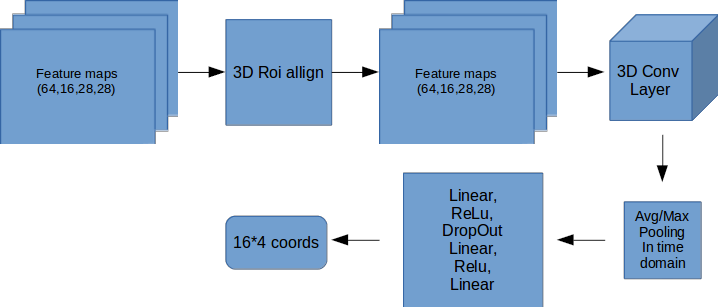
\includegraphics[scale=0.48]{regressor_1_1}
  \caption{Structure of Regressor}
  \label{fig:regressor_3d}
\end{figure}

\begin{figure}[h]

  \centering
  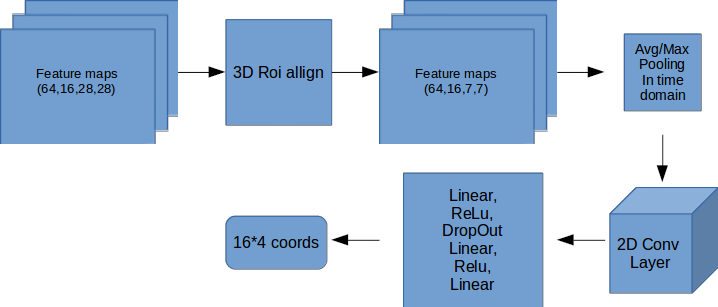
\includegraphics[scale=0.48]{regressor_1_2}
  \caption{Structure of Regressor}
  \label{fig:reg_1_2}
\end{figure}

Η διαδικασία που ακολουθούν και οι δύο Regressors περιγράφεται παρακάτω:
\begin{enumerate}
\item Αρχικά αφού εξάγουμε τα αντίστοιχα feature maps για κάθε ToI χρησιμοποιώντας 3D Roi Align τα κανονικοποιούμε. Μετά, στην πρώτη προσέγγιση τροφοδοτούμε ένα 3D Convolutional Layer με
  kernel ίσο με 1, stride ίσο με 1 και χωρίς padding. Στην συνέχεια, εφαρμόζουμε μια pooling διαδικασία στην διάσταση του χρόνου (είτε avg είτε max pooling). Απ'
  την άλλη, στην δεύτερη προσέγγιση, πρώτα εφαρμόζουμε avg/max pooling στην διάσταση του χρόνου και στην συνέχεια τροφοδοτούμε ένα 2D Convolutional Layer με
  kernel = 1, stride = 1 και χωρίς padding.
\item Και στις δύο περιπτώσεις λαμβάνουμε ως έξοδο ένα feature map με διαστάσεις (64,7,7) το οποίο περνάμε διαδοχικά από 1 γραμμικό layer, 1 Relu Layer, 1 Dropout Layer,
  άλλο ένα γραμμικό Layer, άλλο ένα ReLu layer και ένα τελικό γραμμικό layer. Το τελευταίο layer μας δίνει ως έξοδο 64 στόχους, 4 $\cdot$ 16 μετακινήσεις.
\end{enumerate}


\begin{table}[h]
  \centering
  \begin{tabular} {||c | c || c | c | c ||}
    \hline
    \textbf{Dataset} & \textbf{Pooling} & \textbf{Cuboid} & \textbf{Singl. Fr. } &  \textbf{Follow-up S.F.}\\
    \hline                
    \multirow{2}{*}{JHMDB} & avg & 0.8545 & 0.7649 & 0.7183 \\
    \cline{2-5}
    {} & max & 0.8396 & 0.7761 & 0.5783 \\
    \cline{1-5}
    \multirow{2}{*}{UCF} & avg & 0.5319 & 0.4694 & 0.5754 \\
    \cline{2-5}
    {} & max & 0.5190 & 0.5021 & 0.5972 \\
    \cline{1-5}
                                   
  \end{tabular}
  \caption{Recall results after convertying cuboids into sequences of frames}
  \label{table:reg_1_1}
\end{table}

\begin{table}[h]
  \centering
  \begin{tabular}{||c | c | c || c  c  c ||}
    \hline
    \textbf{Dataset} & \textbf{Pooling} & \textbf{F. Map} & \textbf{Recall} &  \textbf{ Recall SR}  &  \textbf{Recall SRF} \\
    \hline
    \multirow{6}{*}{JHMDB} & \multirow{3}{*}{mean} & 64 &  0.6828  & 0.5112  & 0.7610 \\
    \cline{3-6}
    {} & {} & 128 & 0.8694 & 0.7799 & 0.6756 \\
    \cline{3-6}
    {} & {} & 256 & 0.8396 & 0.7687 & 0.7029 \\
    \cline{2-6}
    {} & \multirow{3}{*}{max} & 64 &  0.8582 & 0.7985 & 0.5914\\
    \cline{3-6}
    {} & {} & 128 & 0.8358 & 0.7724 & 0.8118 \\
    \cline{3-6}
    {} & {} & 256 & 0.8657 & 0.8022 & 0.7996 \\
    \hline
    \multirow{6}{*}{UCF} & \multirow{3}{*}{mean} & 64 & 0.5055 & 0.4286 & 0.5889 \\
    \cline{3-6}
    {} & {} & 128 & 0.5335 & 0.4894 & 0.5893 \\
    \cline{3-6}
    {} & {} & 256 & 0.5304 & 0.4990 & 0.6012 \\
    \cline{2-6}
    {} & \multirow{3}{*}{max} & 64 & 0.5186 & 0.4990 & 0.5708 \\
    \cline{3-6}
    {} & {} & 128 & 0.5260 & 0.4693 & 0.5513 \\
    \cline{3-6}
    {} & {} & 256 & 0.5176 & 0.4878 & 0.6399 \\
    \hline

  \end{tabular}
  \caption{Recall performance using 3 different feature maps as Regressor's input and 2 pooling methods}
  \label{table:reg_1_2}
\end{table}

Οι πίνακες \ref{table:reg_1_1} και \ref{table:reg_1_2} περιέχουν τα αποτελέσματα για την πρώτη και δεύτερη προσέγγιση. Μάλιστα, για την δεύτερη προσέγγιση ελεγξαμε 3 διαφορετικούς χάρτεσ
χαρακτηριστικών, ενώ και στις 2 περιπτώσει πειραματιστήκαμε χρησιμοποιοώντας και τις 2 προαναφερθέντες pooling μεθόδους για τα σύνολα δεδομένων JHMDB και UCF-101. Παρατηρούμε ότι,
Με βάση τα παραπάνω αποτελέσματα, λαμβάνουμε σχετικά χαμηλή recall απόδοση για το dataset UCF ενώ για το JHMDB τα αποτελέσματα είναι κάπως καλύτερα. Πιο συγκεκριμένα, με βάση την πρώτη
προσέγγιση λαμβάνουμε τελικά recall απόδοση ίση με 76-77\% για το JHMDB και 46-50\% για το UCF. Με βάση την δεύτερη προεγγιση, στην καλύτερη περίπτωση λαμβάνουμε 80\% απόδοση recall για
το JHMDB ενώ για το UCF παραμένουμε στα ίδια περίπου αποτελέσματα. Παράλληλα παρατηρούμε ότι χάνουμε περίπου 30-40\% από τις καλές cuboid προτάσεις και στις 2 περιπτώσεις, το οποίο αποτελεί μεγάλο
πρόβλημα και των δύο προσεγγίσεων. Όλ' αυτά μας κάνουν να ξανασκεφτούμε τον τρόπο που σχεδιάσαμε το TPN.


\section{Τα τριασδιάστατα anchors ως 4k διανύσματα}
Σε αυτή την προσέγγιση, ορίζουμε τους 3D anchors ως διανύσματα με 4k συντεταγμένες (k = 16 καρέ = διάρκεια δείγματος). Έτσι ένα τυπικό anchor γράφεται ως ($x_1, y_1, x'_1, y'_1, x_2, y_2, ...$)
όπου $x_1, y_1, x'_1, y'_1 $ είναι οι συντεταγμένες για 1ο καρέ, $x_2, y_2, x'_2, y'_2$ για το 2ο καρέ κλπ, όπως παρουσιάστηκε από τους \cite{DBLP:journals/corr/abs-1712-09184}. 
Η εικόνα \ref{fig:anchor_4k} απεικονίζει ένα τέτοιου τύπου anchor.

\begin{figure}[h]
  \centering
  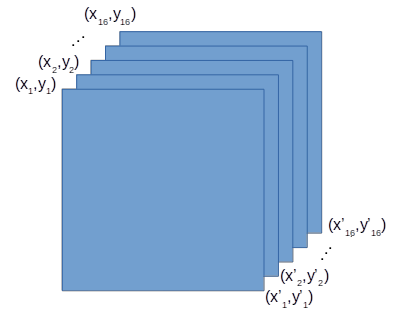
\includegraphics[scale=0.5]{anchor_4k}
  \caption{An example of the anchor $(x_1,y_1,x'_1,y'_1,x_2,y_2, ...)$}
  \label{fig:anchor_4k}
\end{figure}

Το κύριο πλεονέκτημα αυτής της προσέγγισης είναι ότι δεν χρειάζεται να μεταφράσουμε τα 3D anchors  σε 2D κουτιά, γεγονός που προκάλεσε πολλά προβλήματα στην προηγούμενη προσέγγιση.
Ωστόσο,αυτή η προσέγγιση έχει ένα μεγάλο μειονέκτημα, το οποίο είναι το γεγονός ότι αυτός ο τύπος anchor έχει σταθερή χρονική διάρκεια.
Για να ασχοληθούμε με αυτό το πρόβλημα, έχουμε ορίσει anchors με διαφορετικές χρονικές διάρκειες, οι οποίες είναι 16, 12, 8 και 4.
Anchors με διάρκεια $<$  διάρκεια του δείγματος (16 καρέ) μπορούν  να γραφτούν ως διάνυσμα 4k με μηδενιστικές συντεταγμένες στα καρέ μεγαλύτερα από τη χρονική διάρκεια. Για παράδειγμα, ένα anchor με
2 καρέ διάρκεια, ξεκινώντας από το 2ο πλαίσιο και τερματίζοντας στον 3ο μπορεί να γραφεί ως (0, 0, 0, 0, $x_1, y_1, x'_1, y'_1, x_2, y_2, x'_2, y'_2$, 0, 0, 0, 0)  εάν η διάρκεια δείγματος
 είναι 4 καρέ. 

\begin{figure}[h]
  \centering
  % 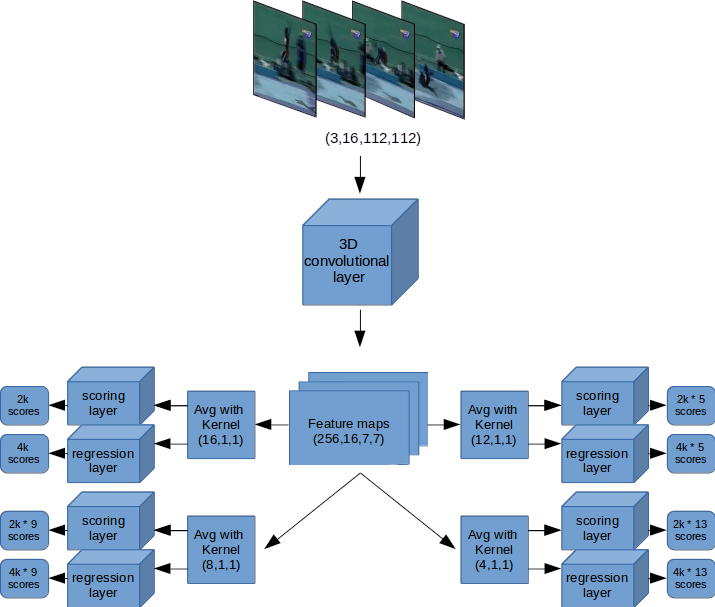
\includegraphics[width=1.\textwidth]{tpn_2}
  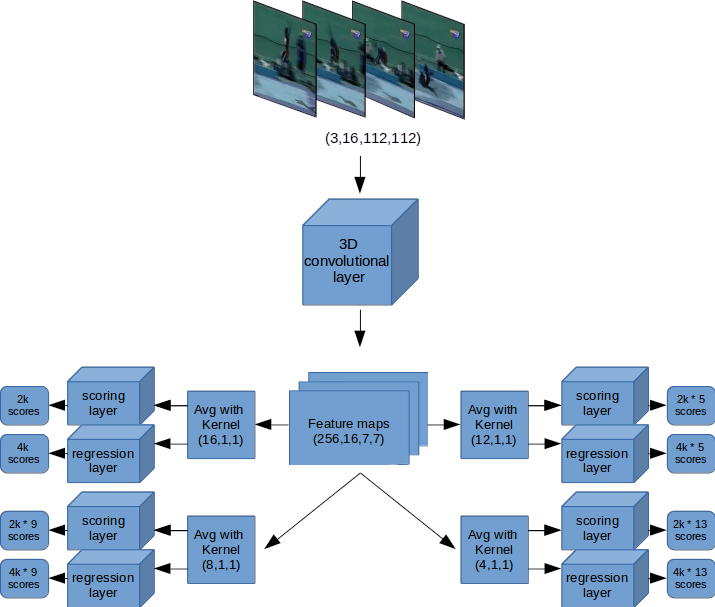
\includegraphics[scale=0.4]{tpn_2}
  \caption{The structure of TPN according to new approach}
  \label{fig:New_structure}
\end{figure}
Αυτή η νέα προσέγγιση μας οδήγησε στο να αλλάξουμε την δομή του TPN. Η νέο δομή του απεικονίζεται στην εικόνα  \ref{fig:New_structure}. Όπως
μπορούμε να δούμε, προσθέσαμε scoring και regression layers για κάθε διάρκεια. Έτσι, το TPN ακολουθεί τα επόμενα βήματα για να παράγει ToIs.
\begin{enumerate}
\item Στην αρχή, τροφοδοτούμε τον χάρτη χαρακτηριστικών, που εξάγεται από το 3D ResNet34, ως είσοδο σε ένα 3D Convolutional Layer με μέγεθος πυρήνα = 1, stride = 1 και χωρίς padding.
\item Από το Convolutional Layer, έχουμε ως αποτέλεσμα ένα χάρτη ενεργοποίησης με διαστάσεις (256, 16, 7, 7). Για τη μείωση της χρονικής διάστασης, χρησιμοποιούμε 4 pooling layers,
  ένα για κάθε δείγμα διάρκειας με μεγέθη πυρήνα  \textit{(16, 1, 1), (12, 1, 1,), (8, 1, 1) και (4, 1, 1)} και stride = 1, για τη διάρκεια του δείγματος 16, 12, 8 και 4 αντίστοιχα.
  Έτσι, έχουμε χάρτες ενεργοποίησης με διαστάσεις \textit{(256, 1, 7, 7), (256, 5, 7, 7), (256, 9, 7, 7) και (256, 13, 7, 7)}, στης oποίες η δεύτερη διάσταση είναι ο αριθμός των πιθανών
  χρονικές διακυμάνσεων. Για παράδειγμα, σε  χάρτη χαρακτηριστικών με διαστάσεις $(256, 5, 7, 7)$, το οποίο σχετίζεται με anchors με διάρκεια 12 καρέ, μπορούμε να έχουμε 5 πιθανές περιπτώσεις,
  από το καρέ 0 μέχρι το καρέ 11, από το καρέ 1 μέχρι το καρέ 12 κλπ.
  
\item Ξανά, όπως και στην προηγούμενη προσέγγιση, για κάθε pixel του χάρτη ενεργοποίησης αντιστοιχούμε \textbf{n = k = 15}
  anchors (5 κλίμακες από 1, 2, 4, 8, 16, και 3 aspect ratios 1:1, 1:2, 2:1). Φυσικά, έχουμε 4 διαφορετικούς χάρτες ενεργοποίησης, με 1, 5, 9 και 13
  διαφορετικές περιπτώσεις και ένα $7  \times 7$ σχήμα σε κάθε φίλτρο. Έτσι, συνολικά έχουμε $28  \cdot 15 \cdot 49 = 20580$ διαφορετικά anchors.
  Αντίστοιχα, έχουμε 20580 διαφορετικούς στόχους regression.

\end{enumerate}

% \subsection{Training}
% Η διαδικασία κατάρτισης παραμένει σχεδόν η ίδια όπως και η προηγούμενη προσέγγιση. Έτσι, και πάλι, εμείς τυχαία επιλέγουμε ένα τμήμα βίντεο και θεωρούμε άγκυρες με επικάλυψη μεγαλύτερη από 0,8 με οποιαδήποτε επίγεια αλήθεια
% σωλήνα, μαζί με άγκυρες παρασκηνίου των οποίων η επικάλυψη είναι μεγαλύτερη που 0,1 και μικρότερη από 0,3.

% \begin{table}[h]
%   \centering
%   \begin{tabular}{||c | c || c  c c||}
%     \hline
%     \textbf{Dataset} & \textbf{Pooling} &  \textbf{Recall(0.5)} & \textbf{Recall(0.4)} & \textbf{Recall(0.3)} \\
%     \hline  \hline
%     \multirow{2}{4em}{JHMDB} & mean & 0.6866 & 0.7687 & 0.8582 \\
%     \cline{2-5}
%     {} & max &  0.8134 & 0.8694 & 0.9216 \\
%     \hline
%     \multirow{2}{4em}{UCF} & avg &  0.5435 & 0.6326 & 0.7075 \\
%     \cline{2-5}
%     {} & max & 0.6418 & 0.7255 & 0.7898 \\
%     \hline
%   \end{tabular}
%   \caption{Recall results using 2nd approach for anchors}
%   \label{table:tpn_2_1}
% \end{table}

% Ως πίνακας  REF{Table: tpn_2_1}, είναι προφανές ότι έχουμε καλύτερες επιδόσεις ανάκλησης σε σύγκριση με την προηγούμενη προσέγγιση.
% Επιπλέον, μπορούμε να δούμε ότι 3Dmax ομαδοποίηση αποδίδει καλύτερα από 3D μέση ομαδοποίηση. Η διαφορά
% μεταξύ της μέγιστης ομαδοποίησης και της μέσης συγκέντρωσης είναι περίπου 10 %, η οποία είναι αρκετά μεγάλη για να μας κάνει να επιλέξουμε μέγιστη λειτουργία ομαδοποίησης πριν από τη λήψη βαθμολογίας άγκυρες
% και τους στόχους παλινδρόμησης.

% \subsection{Adding regressor}

% Ακόμα και αν, η TPN μας εξάγει κουτιά σε επίπεδο πλαισίων, πρέπει να βελτιώσουμε αυτές τις προβλέψεις προκειμένου να αλληλοεπικαλύπτονται
% με τα κουτιά της αλήθειας όσο το δυνατόν καλύτερα.
% Έτσι, σε πλήρη αντιστοιχία με την προηγούμενη προσέγγιση, προσθέσαμε μια παλινδρόμηση για να προσπαθήσουμε να πάρουμε καλύτερα αποτελέσματα ανάκλησης.

% \paragraph{3D Roi align}
% Σε αυτή την προσέγγιση, γνωρίζουμε ήδη τις συντεταγμένες 2D. Έτσι, μπορούμε να χρησιμοποιήσουμε τη μέθοδο που προτείνεται στο cite{DBLP: εγγραφές/Corr/ABS-1712-09184}. Είναι
% επέκταση του χειριστή με διαχωρισμό του σωλήνα σε κουτιά $T $2D. Στη συνέχεια, χρησιμοποιούν κλασικό Ρόροστοίχιση για να εξαγάγετε μια περιοχή από κάθε
% των χρονικών slice στον χάρτη δυνατοτήτων. Μετά από αυτό, συνδέονται με την περιοχή στον τομέα του χρόνου, ώστε να έχουν μια $T$ servesr sr$ R $
% χαρακτηριστικό χάρτη, όπου $R $ είναι η ανάλυση εξόδου του Ροροστοιχίστε, το οποίο είναι 7 στην περίπτωσή μας.  par

% Ως πρώτη προσέγγιση, χρησιμοποιούμε ένα επίπεδο convolutional 3D ακολουθούμενο από 2 γραμμικά στρώματα. Οι αντιστάσεις μας ακολουθούν τα ακόλουθα βήματα:
% \begin{enumerate}
% \item Στην αρχή, χρησιμοποιήστε 3D Ροδοστοίχιση για να εξαγάγετε τους χάρτες δυνατοτήτων των προτεινόμενων σωλήνων δράσης. Τα ομαλοποιήσαμε και τα δίνουμε ως εισαγωγή στο 3D
%   convolutional στρώση.
% \item Η έξοδος του 3D Convolutional Layer τροφοδοτείται σε 2 γραμμικά στρώματα με τη φατρία ReLu μεταξύ τους και τελικά έχουμε $sample διάρκεια  φορές $4
%   στόχους παλινδρόμησης. Κρατάμε μόνο τους προτεινόμενους στόχους, ότι υπάρχει ένα αντίστοιχο κουτί 2D.
% \end{enumerate}

% Εκπαιδεύουμε την παλινδρόμηση μας χρησιμοποιώντας την ίδια λειτουργία απώλειας όπως ο τύπος της προηγούμενης προσέγγισης που είναι:
% \begin{equation*} 
% \begin{split}
%  L  =  \sum_iL_{cls}(p_i, p_i^*) + \sum_iL_{cls}(p_{fixed,i}, p_{fixed,i}^*) + \\
%  \sum_ip_i^*L_{reg}(t_i,t_i^*) + \sum_ip_{fixed,i}^*L_{reg}(t_{fixed,i},t_{fixed,i}^*) + \\
%   \sum_iq_i^*L_{reg}(c_{i}, c_{i}^*) + \\
%   % \sum_iL_{cls}(p_i, p_i^*) + \sum_iL_{cls}(p_{fixed,i}, p_{fixed,i}^*) 
% \end{split}
% \end{equation*}


\end{document}